%%%%%%%%%%%%%%%%%%%%%%%%%%%%%%%%%%%%%%%%%%%%%%%%%%%%%%%%%%%%%%%%%%%%%%
\section{Casper Design Overview}\label{sec:des-basic}
%%%%%%%%%%%%%%%%%%%%%%%%%%%%%%%%%%%%%%%%%%%%%%%%%%%%%%%%%%%%%%%%%%%%%%
In our previous work, we have proposed ``Casper'', a process-based
asynchronous progress model that provides static asynchronous progress
configuration for MPI one-sided communication~\cite{casper}.
In this section, we summarize its basic design and discuss the shortcoming.

Casper is designed as an external library through the PMPI name-shifted
profiling interface of MPI. This allows Casper to transparently link with
various MPI implementations, by overloading the necessary MPI functions.
The basic implementation of Casper can be summarized into four parts:
\begin{enumerate}
\item At MPI initialization stage, a few user defined number of cores are
kept aside as the background ``ghost processes'', which are hidden from
the user application by replacing the \fn{MPI\_COMM\_WORLD} with a
subcommunicator \fn{COMM\_USER\_WORLD} that only consists of user processes
in all MPI calls.

\item When the user processes try to allocate a remotely accessible window
by using \fn{MPI\_WIN\_ALLOCATE} function, Casper internally allocate a
shared-memory window for each user process and the ghost processes on
the same node using MPI-3 \fn{MPI\_WIN\_ALLOCATE\_SHARED} function. Thus
the ghost processes are allowed to access the user window region located
in the memories of the user processes.

\item Whenever the user process (P0) tries to issue an RMA operation or
an RMA synchronization (i.e., lock, fence, post-start-complete-wait) to
a target process (P1), Casper transparently redirects this message to
the corresponding ghost process of P1 through PMPI redirection as shown
in Figure~\ref{fig:des-casper-async}.

\item The ghost processes simply wait in an \fn{MPI\_RECV} loop to receive
any requests (e.g., allocate window ) from the local user processes, thus
allowing the MPI implementation to make progress on any RMA communication
targeted to those ghost processes.
\end{enumerate}

\begin{figure}
  \subfigure[Original Accumulate.] {
    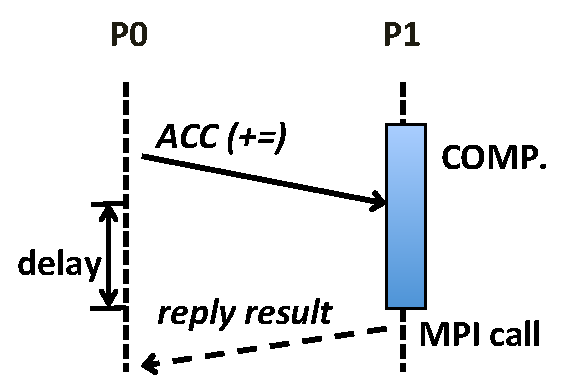
\includegraphics[height=0.31\columnwidth]{figures/adpt-casper/design-casper-async-orig.pdf}
    \label{fig:des-casper-async-orig}
  }
  \hfill
  \subfigure[Accumulate with Casper.] {
    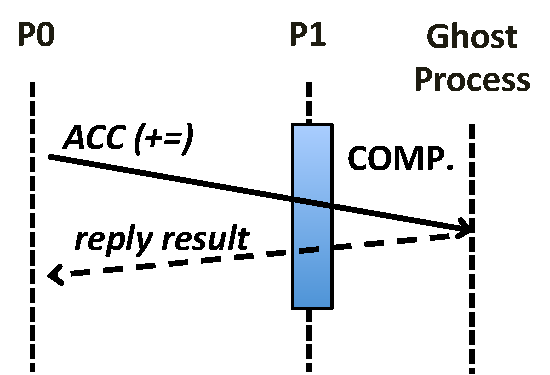
\includegraphics[height=0.31\columnwidth]{figures/adpt-casper/design-casper-async-casper.pdf}
    \label{fig:des-casper-async-async}
  }
  \vspace{-1.0ex}
  \caption{RMA asynchronous progress.}
  \label{fig:des-casper-async}
  \vspace{-3.0ex}
\end{figure}

The static operation redirection allows Casper to provide efficient
asynchronous progress for software-handled RMA operations without
effect the performance of any hardware-handled operations (e.g., contiguous
PUT/GET operations on RDMA supported network).
However, such static redirection may not be sufficient for some large
applications that always compose of multiple internal phases with
different proportion of communication.
That is, in communication-sparse phases, the ability of asynchronous
progress is important because arbitrary long delay can happen when the
target processes are so busy in computing that cannot make MPI progress;
in communication-intensive phases, however, the asynchronous progress may
not be necessary because the target processes can frequently make MPI calls
and thus handle the operations issued to them as targets by themselves.
Furthermore, when the amount of RMA operations becomes large, redirecting
operations to a few of ghost processes may even result in performance
degradation in communication, since those operations were originally
distributed to many user target processes (the number of user process
is always much larger than the amount of ghost processes). We will
demonstrate such inefficiency in the quantum chemistry application
NWChem in Section~\ref{sec:eva-nwchem}.

To distinguish with the adaptable version, we use static Casper to
indicate the basic version with static configuration of asynchronous
progress in the remainder of this paper.

